\section{Introduction}
\label{sect:introduction}

Supersymmetry (SUSY) \cite{Golfand:1971iw,Wess:1973kz,Wess:1974tw,Fayet1,Fayet2} is one of the most promising extensions of the 
standard model (SM) of elementary particles.  It leads to the unification of gauge couplings at
high energy, mitigates the problem of quadratic divergences in quantum corrections to the
mass of the Higgs boson, and, in its R-parity realization, provides a dark matter candidate.
A key prediction of SUSY is the existence of new particles with the same quantum numbers as SM particles but
differing in mass and by half-a-unit in spin (``sparticles'').

Extensive searches at the CERN LHC during the Run 1 have excluded the existence of colored sparticles with masses below a few hundred \GeV to about 1.8\TeV,
depending on the details of the assumed models~\cite{%Chatrchyan:2012paa,Chatrchyan:2013xna,Chatrchyan:2013wxa,
Chatrchyan:2013fea,Chatrchyan:2013mys,Chatrchyan:2014aea,Chatrchyan:2014lfa,%Khachatryan:2015exa,
Khachatryan:2015vra,Khachatryan:2015lwa,Aad:2015pfx,Aad:2015iea}. %\cite{susyPhyRes}.
On the other hand, the constraints on sparticles with only electroweak quantum numbers are much less stringent.  This motivates the electroweak SUSY search 
described in this paper.


Searches for charginos ($\widetilde{\chi}^{\pm}\xspace$), neutralinos ($\widetilde{\chi}^{0}\xspace$), and sleptons ($\widetilde{\ell}\xspace$) by the ATLAS and CMS Collaborations are described in Refs.~\cite{Aad:2014nua,Aad:2014vma,Khachatryan:2014qwa,Khachatryan:2014mma,Khachatryan:2015kxa}.
In various SUSY models, the lightest SUSY partners of SM fermions are those of third generation, 
resulting in enhanced branching fractions for final states with $\tau$ leptons~\cite{Martin:1997ns}.  
%Here we report on a search for new physics in events with two $\tau$ leptons and missing transverse momentum (\MPT), i.e., final states that were not explicitly targeted in the previous publications.
The previous searches for charginos, neutralinos,
and sleptons by the CMS collaboration  
 either did not include the possibility that 
the scalar $\tau$ lepton and its neutral partner (\stau and $\sNu_\tau$) 
are the lightest sleptons \cite{Khachatryan:2014qwa}, or the initial charginos and neutralinos are produced in vector-boson fusion processes \cite{Khachatryan:2015kxa}. An ATLAS search for SUSY in the di-$\tau$ channel is reported in Ref. \cite{Aad:2014yka}, excluding chargino masses up to 345 \GeV 
for a massless neutralino (\PSGczDo).


In this paper, a search for the lightest charginos (\chione) is reported using events 
with two opposite-sign $\tau$ leptons and 
missing transverse momentum (\MPT), assuming the masses of the third-generation sleptons are between those of the 
chargino and the lightest neutralino. 
Two $\tau$ leptons can be generated in the decay chain of \chione and \sTau, as shown in Fig.~\ref{fig:Productions}. 
\begin{figure}[!htb]
\centering
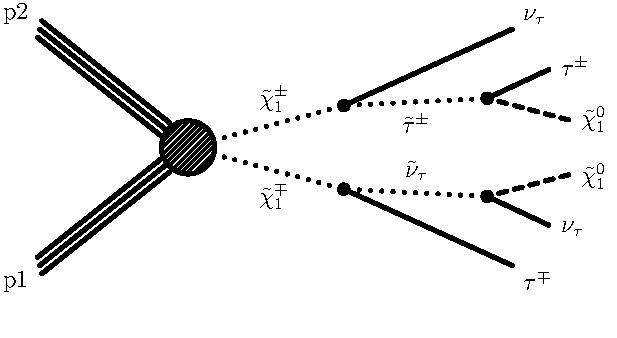
\includegraphics[width=0.45\textwidth]{Introductionfigs/TChipmSlepSnu.pdf}
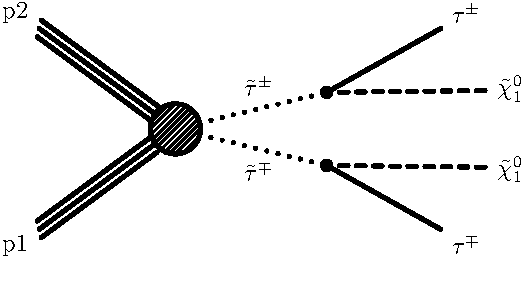
\includegraphics[width=0.41\textwidth]{Introductionfigs/TSlepSlep.pdf}

\caption{Schematic production of $\tau$ lepton pairs from chargino (left) or $\tau$ slepton (right) pair production.}
\label{fig:Productions}
\end{figure}
%Figure \ref{fig:Productions} shows a representative diagram of pair production of charginos in such a final state. 
The results of the search are interpreted in the context of SUSY simplified model spectra (SMS) \cite{Alwall:2008ag,alves:sms} for both
production mechanisms.


The results discussed here are based on a data set of proton-proton 
collisions at $\sqrt{s}$ = 8\TeV
collected with the CMS detector at the LHC during 2012, corresponding to integrated
luminosities of 18.1 and 19.6 \invfb in different channels. 
This search makes use of the ``stransverse mass'' variable (\mttwo)~\cite{Lester:1999tx,Barr:2003rg},
which is the extension of transverse mass (\mt) to the case 
where two massive particles with equal mass are created in pairs  
and decay to two invisible particles accompanied by two $\tau$ leptons.  
The distribution of \mttwo reflects the scale of the produced particles and has a longer tail for heavy sparticles
compared to lighter SM particles. Hence, SUSY 
can manifest itself
as an excess of events in the high-side tail of the \mttwo distribution. 
Final states are considered where
two $\tau$ leptons are each reconstructed via hadronic decays (\tauTau), or where only one $\tau$ lepton is reconstructed as the \Tau and the other decays leptonically (\leptonTau, where $\ell$ is an electron or muon). 
% as a hadronic decay of a $\tau$ (\tauTau), or where only one tau lepton is reconstructed as the hadronic decay of a $\tau$ and the other one decays leptonically (\leptonTau;~ $\ell=$ electron or muon).

The paper is organized as follows.  The CMS detector, the event reconstruction, and the data sets are described
in Sections \ref{sect:CMSRec} and \ref{sect:MCSamples}; the \mttwo variable is introduced in Section \ref{sect:mt2def}; 
the selection criteria for the \tauTau and \leptonTau channel are described in Section \ref{sect:tauTauCuts} and \ref{sect:eleTauCuts}, respectively;
a detailed study of the SM backgrounds is presented in Section \ref{sect:bkg}, while Section \ref{sect:sys} 
is devoted to the description of the systematic uncertainties.  The results of the search with its statistical interpretation is presented in 
Section \ref{sect:stat}. The efficiencies for the important selection criteria are summarized in Section \ref{sect:model} and can be
used to interpret these results within other phenomenological models. Conclusions are given in Section \ref{sect:conclusion}.
%and the paper is finally summarized in Section \ref{sect:conclusion}.



